\subsubsection{Controller}

\rule{\textwidth}{0.4pt}
\class{AngularController}
public class AngularController

\begin{minipage}{0.4\textwidth}
    \begin{figure}[H]
        {\centering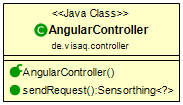
\includegraphics[scale = 0.7]{media/frontend/controller/AngularController_Class.png}}
    \end{figure}
    \end{minipage} \hfill
    \begin{minipage}{0.6\textwidth}
Der AngularController stellt Anfragen an das Backend und wandelt die erhaltenen JSON Dateien in Sensorthings um. Dieser wird mithilfe des jsweet-Angular-4 Candies implementiert und erleichtert so die Kommunikation zwischen backend und frontend.
\end{minipage}
Methoden: \begin{itemize}
    \item \emph{public synchronized Sensorthing sendRequest(String input)} Eine synchrone Anfrage an das Backend auf dem Server welche die gewünschten Daten abfragt und diese dann dem Benutzer anzeigt.
\end{itemize}